
\begin{figure}
  \setlength{\fboxsep}{0pt} % box tighlty around text
  \begin{subfigure}{0.48\textwidth}
    \fbox{% frame
      \adjustbox{valign=B}{% margins
        \resizebox{\textwidth}{!}{% scale
          \lstinputlisting[
            basicstyle=\scriptsize\sffamily,
            language=sparql, numbers=none, columns=flexible,
            commentstyle=\color{Gray!70},
            showstringspaces=false]{
            figures/query-q1-j2-no-star.rq
      } } } }
    \caption{\label{fig:q1-j2-1hop}Query $Q_1$: All cycling races of Central America along
      with their respective country.}
  \end{subfigure}
  \hfill
  \begin{subfigure}{0.48\textwidth}
    \fbox{%
      \resizebox{\textwidth}{!}{% scale
        
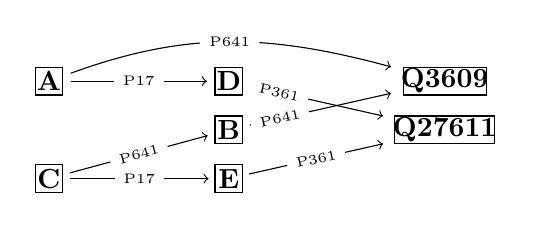
\begin{tikzpicture}

  \thickmuskip=0mu
  \medmuskip=0mu
  \thinmuskip=0mu

  \newcommand\X{65pt}
  \newcommand\Y{-17.6pt}
  \newcommand\PREDICATE{\tiny}
  
  \draw (0, 0) node(A){\textbf{A}} +(-5pt, -5pt) rectangle +(5pt, 5pt);
  \draw (\X, 0) node(D){\textbf{D}} +(-5pt, -5pt) rectangle +(5pt, 5pt);
  \draw (2.2*\X, 0) node(Q3609){\textbf{Q3609}} +(-15pt, -5pt) rectangle +(15pt, 5pt);

  \draw (\X, \Y) node(B){\textbf{B}} +(-5pt, -5pt) rectangle +(5pt, 5pt);
  \draw (2.2*\X, \Y) node(Q27611){\textbf{Q27611}} +(-18pt, -5pt) rectangle +(18pt, 5pt);
  \draw (0, 2*\Y) node(C){\textbf{C}} +(-5pt, -5pt) rectangle +(5pt, 5pt);
  \draw (1*\X, 2*\Y) node(E){\textbf{E}} +(-5pt, -5pt) rectangle +(5pt, 5pt);
  

  \draw[->] (A) -- node[fill=white, font=\PREDICATE]{P17} (D);
  \draw[->] (C) -- node[fill=white, sloped, font=\PREDICATE]{P641} (B);
  \draw[->] (C) -- node[fill=white, sloped, font=\PREDICATE]{P17} (E);
  \draw[->] (B) -- node[fill=white, sloped, font=\PREDICATE, xshift=-1.5em]{P641} (Q3609);
  \draw[->] (E) -- node[fill=white, sloped, font=\PREDICATE]{P361} (Q27611);
  \draw[->] (D) -- node[fill=white, sloped, font=\PREDICATE, xshift=-1.4em]{P361} (Q27611);
  \draw[->] (A) to[out=20, in=165] node[fill=white,sloped, font=\PREDICATE]{P641} (Q3609);
  
  

\end{tikzpicture}

    }}
    % 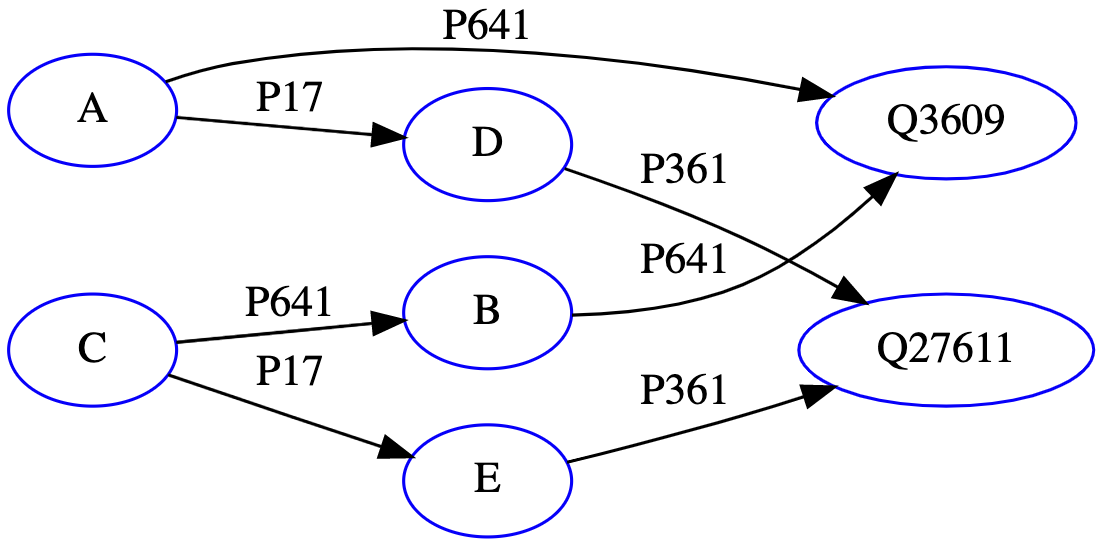
\includegraphics[width=\textwidth]{figures/graph-g1.png}
    \caption{RDF Graph $G_1$: $A$, $B$, and $C$ are cycling sports; $D$ and $E$
      are countries of Central America~\cite{10.1007/978-3-031-33455-9_3}}
  \end{subfigure}
  \caption{\label{fig:random_walks_example}Query $Q_1$ evaluated on
    the RDF graph $G_1$ provides cardinality insights~\cite{10.1007/978-3-031-33455-9_3}.}
\end{figure}

\section{\NAME: RAndom Walks for Apache Jena}
\label{sec:proposal}

\paragraph{Sampling principles.}

%\NAME is based on WanderJoin\cite{li2019wanderjoin}.
Let $Q$ be a SPARQL conjunctive query, and $J = \langle tp_1, ..., tp_n \rangle$ be
the join order to perform random walks. A random walk
$\gamma_i = \langle t_1, ..., t_n\rangle$ is computed over
an RDF graph $G$ by randomly picking $t_1$ in $\llbracket tp_1 \rrbracket_G$,
and each subsequent $t_i$ ($i > 1$) in $\llbracket t_{i-1} \bowtie tp_i \rrbracket_G$.
Once computed, the cardinality of $Q$ is estimated as  the inverse probability
of sampling $\gamma_i$~\cite{li2019wanderjoin}, with $P(\gamma_i) = |\llbracket tp_1 \rrbracket_G|^{-1} \prod_{i=2}^{n}
|\llbracket t_{i-1} \bowtie tp_i \rrbracket_G|^{-1}$.
%
For instance, let us consider the query $Q_1$ and the RDF graph $G_1$
depicted in Figure~\ref{fig:random_walks_example}. Following the join order $tp_3,tp_2,tp_1$, the random walk $\gamma_1$ is computed as
follows:

\begin{small}
  \begin{tabular}{l|lll}
    $tp_3$ & draw  $t_1$ &$= (\textbf{A}, P641, Q3609)$ & $\in \llbracket (?x1, P641, Q3609) \rrbracket_{G_1}$ \\
    $tp_2$ & draw  $t_2$ &$= (A, P17, \textbf{D})$ & $ \in \llbracket (\textbf{A}, P17, ?x3) \rrbracket_{G_1}$  \\
    $tp_1$ & draw  $t_3$ &$= (D, P361, Q27611)$ & $\in \llbracket (\textbf{D}, P361, Q27611) \rrbracket_{G_1}$  
  \end{tabular}
\end{small} 

\noindent The cardinality of $Q_1$ is then estimated as the inverse
probability of sampling $\gamma_1$:

\noindent
\begin{small}
$P(\gamma_1)^{-1}  =  |\llbracket (?x1, P641, Q3609) \rrbracket_{G_1}| \cdot
                          |\llbracket (\textbf{A}, P17, ?x3) \rrbracket_{G_1}| \cdot
                          |\llbracket (\textbf{D}, P361,
                          Q27611) \rrbracket_{G_1}| 
                      =  2 \cdot 1 \cdot 1 = 2$
\end{small}

%% \begin{small}
%% \begin{tabular}{ll}
%%     $P(\gamma_1)^{-1}$  &$=  |\llbracket (?x1, P641, Q3609) \rrbracket_{G_1}| \times
%%                           |\llbracket (\textbf{A}, P17, ?x3) \rrbracket_{G_1}| \times
%%                           |\llbracket (\textbf{D}, P361,
%%                           Q27611) \rrbracket_{G_1}| $ \\
%%                       &$=  2 \times 1 \times 1 = 2$
%% \end{tabular}
%% \end{small}

\noindent Note that a random walk may fail if it becomes impossible to sample $t_i$ for
some $i \leq n$. In this case, its probability $P(\gamma_i)$ of being sampled is 0.
For instance, if $t_1 = (B, P641, Q3609)$ is picked in
$\llbracket (?x1, P641, Q3609) \rrbracket_{G_1}$
instead of $(A, P641, Q3609)$, then the random walk fails because
$\llbracket (B, P17, ?x3) \rrbracket_{G_1} = \varnothing$.
%
To improve the quality of estimates, we compute a set of $k$ random
walks $\Gamma = \langle \gamma_1, ..., \gamma_k \rangle$, and the
cardinality of $Q$ is estimated as
\smash{$|\Gamma|^{-1}\sum_{i=1}^{|\Gamma|} P(\gamma_i)^{-1}$}.


\paragraph{\NAME in action (\url{https://youtu.be/We5-rG6uxN8}).}

% ?x1 <http://www.wikidata.org/prop/direct/P31> <http://www.wikidata.org/entity/Q5> . ?x2 <http://www.wikidata.org/prop/direct/P31> <http://www.wikidata.org/entity/Q5> . ?x1 <http://www.wikidata.org/prop/direct/P569> ?x3 . ?x2 <http://www.wikidata.org/prop/direct/P569> ?x3 . ?x1 <http://www.wikidata.org/prop/direct/P570> ?x4 . ?x2 <http://www.wikidata.org/prop/direct/P570> ?x4 . 

 \begin{figure*}
   \centering
   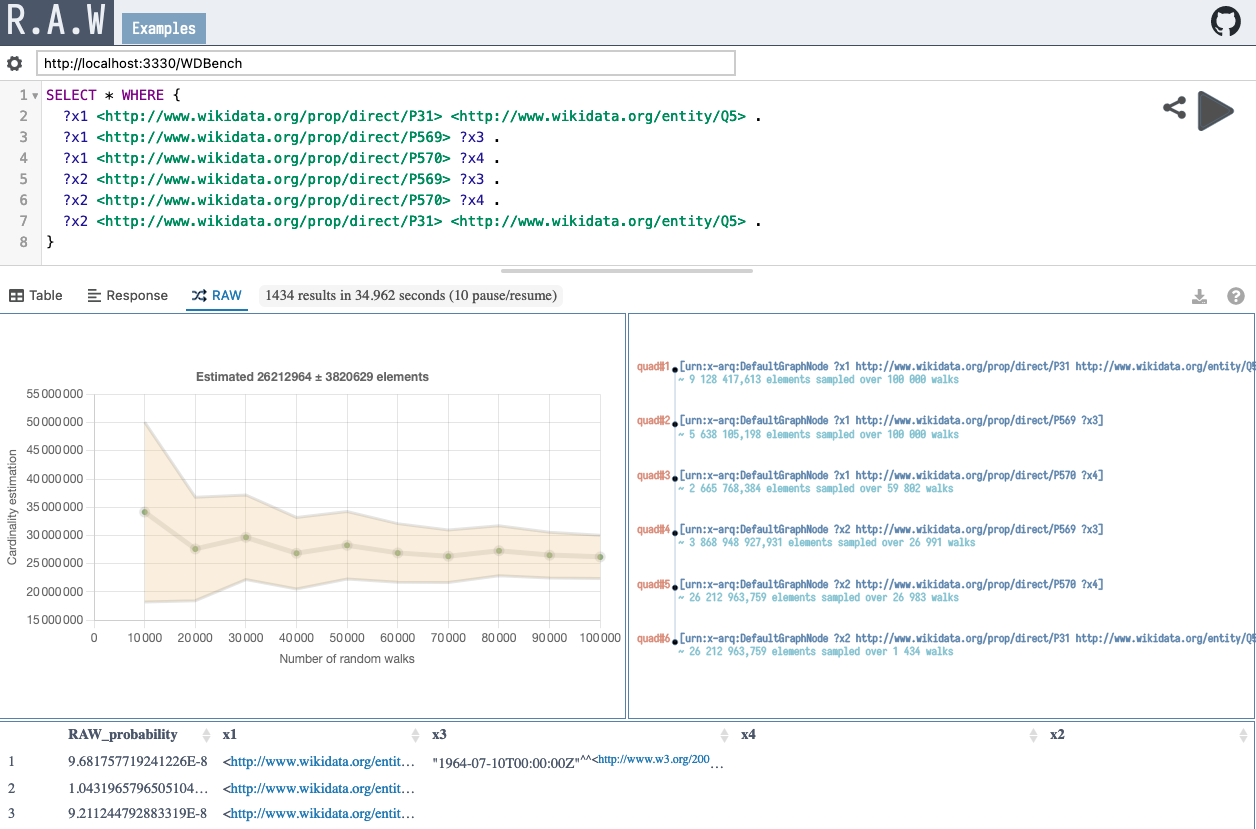
\includegraphics[width=0.91\textwidth]{figures/raw_screenshot.png}
   \caption{\label{fig:raw_screenshot} Screenshot of \NAME processing the query $Q_{604}$ of
     WDBench~\cite{angles2022wdbench}.}
 \end{figure*}

The code is open source and available on the GitHub platform at
\url{https://github.com/Chat-Wane/raw-jena}.  We executed the query
$Q_{604}$ of WDBench~\cite{angles2022wdbench} presented in
Figure~\ref{fig:raw_screenshot} that searches for people with the same
dates of birth and death. $Q_{604}$ expects $25M$ results, but times
out on the public Wikidata SPARQL endpoint after $60$ seconds; and
takes longer than $2$ hours to complete on Apache Jena.


\noindent Each time the user presses the play button, \NAME computes
either $10k$ random walks or as many as possible before reaching $60$
seconds of execution time. By repeating the operation, the web client
merges the results iteratively in a pay-as-you-go fashion.


\noindent The bottom panel of Figure~\ref{fig:raw_screenshot} displays
both succeeded and failed random walks $\gamma_i$ with their
respective probability of being drawn $P(\gamma_i)$.  Increasing the
number of random walks allows for displaying more accurate estimates.  The
left panel of Figure~\ref{fig:raw_screenshot} presents the evolution
of cardinality estimates and confidence intervals with respect to the
number of random walks.  The $1^{st}$ iteration provides a rough
estimate of $35 \pm 15M$ expected results. After $35$ seconds of
execution time and $100k$ random walks, the $10^{th}$ iteration
provides a more accurate estimate of $26 \pm 3M$ of expected results and $1434$ actual random results.
%
The right panel of Figure~\ref{fig:raw_screenshot} displays
the join order with
\begin{inparaenum}[(i)]
\item the estimated cardinality of the partial query up to each
  triple/quad pattern, and
\item the number of random walks that reached each triple/quad pattern.
\end{inparaenum}
Among $100k$ random walks launched on $quad_1$, only $1434$ reached
$quad_6$. This hints that the join order might be suboptimal since
$quad_5$ is very selective and makes random walks fail.


\noindent This example shows how S-AQP can be used for exploratory
queries and optimization. Nevertheless, S-AQP also provides
opportunities for computing large-scale statistics, embeddings, or
summaries.


% %%% Local Variables:
% %%% mode: latex
% %%% TeX-master: "../paper.tex"
% %%% End:
